%!TEX root = ../../dissertation.tex
%%%%%%%%%%%%%%%%%%%%%%%%%%%%%%%%%%%%%%%%%%%%%%%%%%%%%%%%%%%%%%%%%%%%%%%%%%%%%%%%
\section{Measurements}
\label{c3:sec:measurements}

With the buffer-based playback model and strategies at hand, this section demonstrates how to conduct actual evaluations of reliable streaming protocols with it.

As discussed, there are numerous incarnations of reliable streaming protocols in use. Almost all of them follow the same basic approach but every time with slight variations in execution and choice of playback strategies and corresponding parameters. It is exactly these choices that can have a large impact on the streaming process and resulting quality. 

The problem lies in comparing these protocols to each other. Each of them is usually tied to a specific --- and most often proprietary closed source --- streaming player. Setting up all these players in one testbed is a huge effort and requires very specific software environments to be used on the client computers. Moreover, these players are built with user interaction and not automation in mind, hampering efforts of directly measuring the outcome. This can still be achieved through extensive workarounds, but those must be tailored to every individual player application. 

The approach presented here avoids this hassle and provides a concise way to test any conceivable playback strategy in one single test setup.


%%
\subsection{Progressive Streaming Measurement Framework}

To enable quick evaluations for reliable streaming the framework follows a two-phase approach, separating the active online recording phase from the passive playback emulation. Recording network data is very time intensive and cannot be sped up when conducting an investigation of a real world process, and not relying on simulated data. The framework still replicates the steps a user would perform to consume a media stream on a playback device, but simply separates them. Through appropriate configuration different scenarios can be modeled, e.g., network conditions and behavior or specifics of the user device.
 
\begin{figure}[htb]
	\centering
	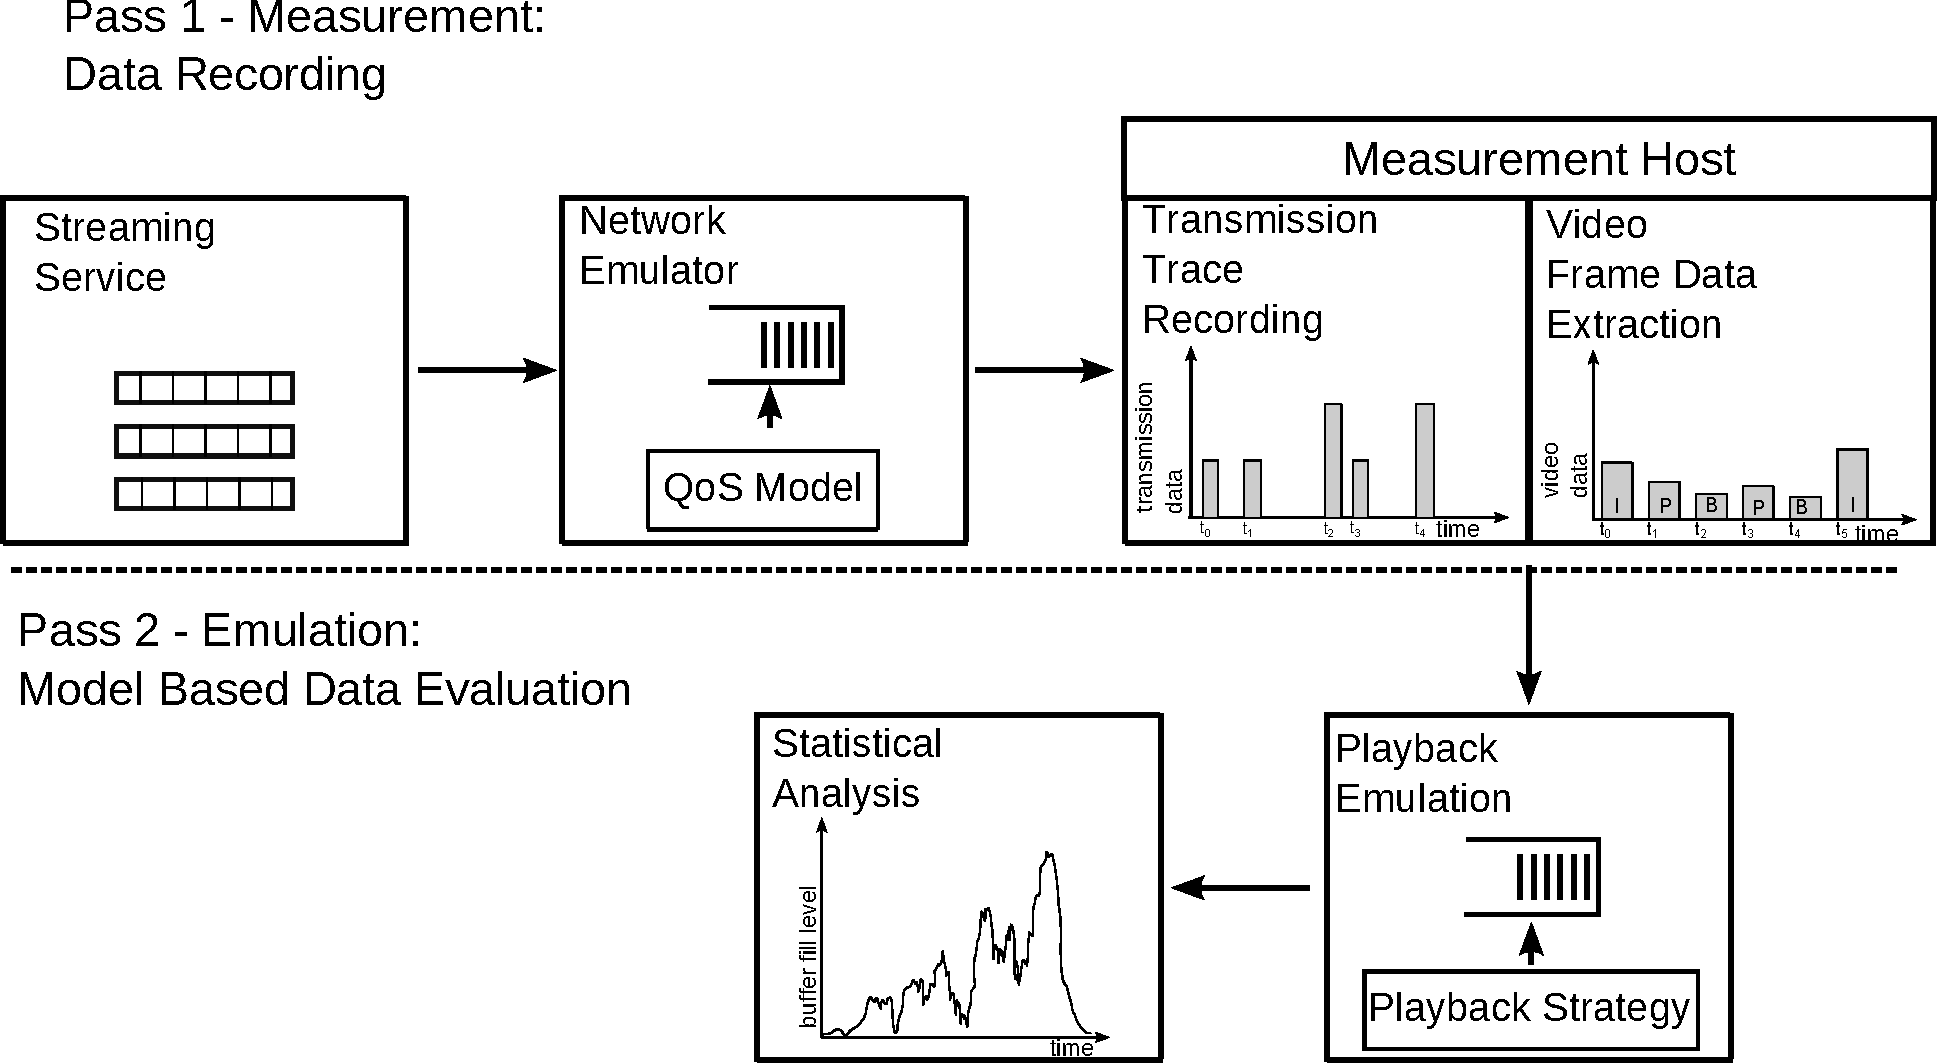
\includegraphics[width=0.9\textwidth]{images/measurement-model.pdf}
	\caption{Overview of the measurement framework for progressive streaming playback strategies.}
\label{c3:fig:framework}
\end{figure}

Figure~\ref{c3:fig:framework} depicts the usage of the framework for a streaming evaluation testbed. In phase one the actual transmission of the stream is conducted and recorded as a packet level network trace. These traces should at least consist of the size and timestamp of every incoming packet.

Stream data is transmitted to the client from a server which can be any actual streaming service on the Internet or a local server under the testbed's control, eliminating undesired side effects caused by the Internet connection. The traffic is further directed through a network emulation node capable of altering the network \gls{QoS} parameters, i.e., latency, jitter, and packet loss. The parameters can be set according to stochastic models derived from actual network architectures such as the \gls{3G} mobile network architecture.

Instead of network emulation, any preexisting architecture can also be placed here to achieve more accurate results for the intended target. This is especially helpful for complex infrastructures hard to model or with no good and concise models available yet. Of special note for this work are the previously discussed mobile networks, which encapsulate the user traffic into tunnels and exhibit complex control plane interactions that can influence the streaming process.

Additionally the received video file is decoded yielding a trace of all video frame sizes and playback timestamps. All data gained in the process is stored as a basis for the second phase. More detailed traces can additionally be used to scrutinize other layers of the connection, e.g., the dynamics of \gls{TCP} receive window size. 

In the second pass, both the network as well as the video data are then used to feed the actual reliable streaming playback model described before. This is conducted by a closed-loop emulation process calculating the current buffer fill level based on the collected transmission and video frame traces for every point in time. 

All of the non-adaptive reliable streaming strategies can be tested on the same trace set. In the simplest form of \gls{HTTP} streaming the transmission is not controlled by the streaming application and no rate control is conducted. Therefore, recording the packet trace and simulating playback are completely decoupled, as the latter cannot influence the former. This enables a fast and efficient comparison of various non-feedback protocols which are all subjected to the same network conditions.

The emulator then generates playback stalling statistics, specifically their number and duration, to compare the effect of the different strategies on the same trace. With these results, parameter settings for playback strategies can also be iteratively tested and improved leading to an empirical calibration of playback strategies instead of relying on best practices.

One of the drawbacks of this model-based emulation approach is of course the reliance on suitable models and playback strategies for the stream protocols under scrutiny. Obtaining these from proprietary closed source streaming clients can be a difficult and time consuming reverse-engineering process.


%%
\subsection{Adaptive Streaming Measurement Framework}

Up to this point, the measurement framework is only suitable for simple reliable streaming strategies but neglects any adaptive strategy. This second iteration of the framework modifies the base framework and allows for the testing of adaptive playback strategies. However, to achieve this, the advantageous two-phase setup cannot be employed anymore.

\begin{figure}[htb]
	\centering
	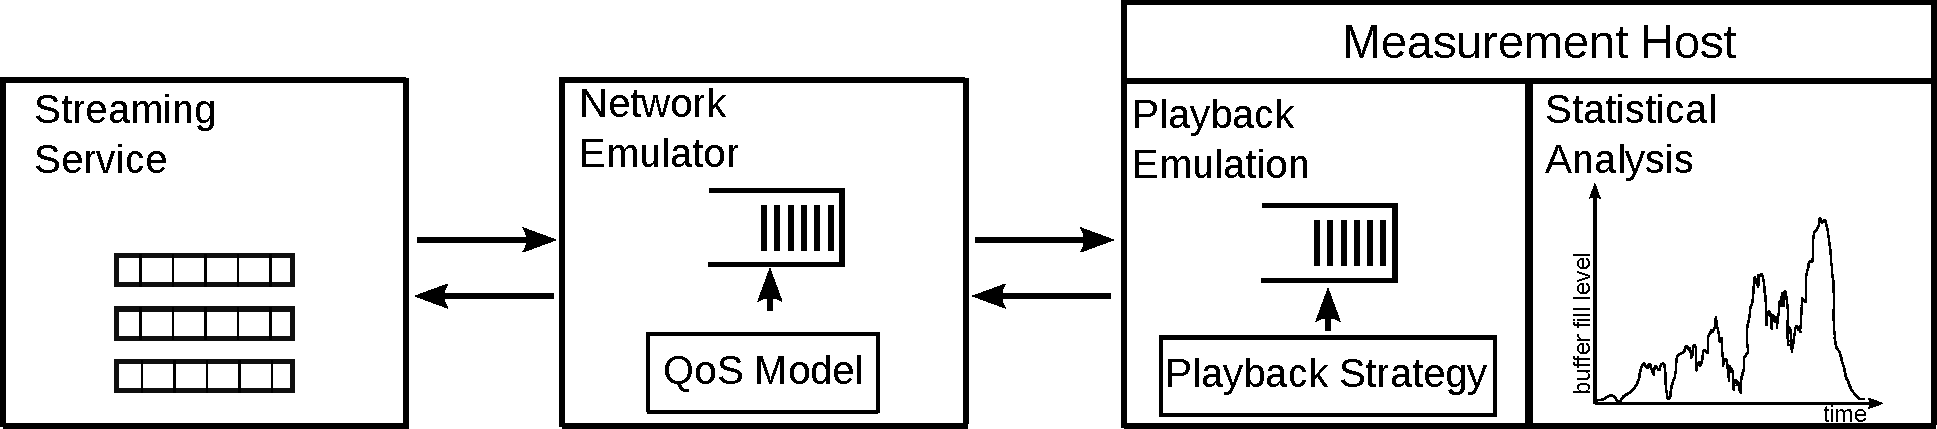
\includegraphics[width=0.9\textwidth]{images/feedback-measurement-model.pdf}
	\caption{Overview of the measurement framework for adaptive streaming playback strategies.}
\label{c3:fig:framework-feedback}
\end{figure}


Figure~\ref{c3:fig:framework-feedback} shows the adapted framework. The playback emulation process is now directly fed with the stream transmission without recording it first. The emulation is now an online process and has to be conducted in realtime. This enables the emulator to react on the current streaming state and request an alteration from the server. The adaptation spectrum ranges from the timing of stream segment retrieval to the chosen quality level of future segments. 

While allowing for a wider range of playback strategies, this approach is also inherently slower as it does not allow a speed-up beyond realtime, limiting its usability somewhat. Therefore, a transition to a full simulative approach is suggested. This is path is further explored and discussed in Section~\ref{c6:sec:mobilestreamingtestbed}.


%%
\subsection{Technical Implementation}

To conduct actual measurements, the described two phase progressive streaming measurement framework has been implemented as a network testbed. The three individual components of the framework in Figure~\ref{c3:fig:framework} are represented by three interconnected physical nodes running Linux. 

The streaming server houses an Apache httpd Web server\footnote{\url{https://httpd.apache.org/}}, hosting the files that are to be streamed. Alternatively, traffic from any viable Internet streaming service can also be directly routed through the network emulation node, making the local streaming server superfluous.

The network emulation node uses existing \gls{QoS} capabilities of the Linux kernel, dubbed NetEm~\cite{hemminger2005network}, to add latency and packet loss to the transmission as well as to act as a bandwidth bottleneck. The additional delay will be set to a deterministic value for the following experiments. The loss follows a uniform distribution without any correlation in the transmission.

Curl\footnote{\url{http://curl.haxx.se/}} is used to both retrieve the streaming file and record the transmission process at the client node. If so desired, tcpdump\footnote{\url{http://www.tcpdump.org/}} can also be facilitated to achieve a higher recording precision. The video file is then parsed for its frame timings and sizes using mplayer\footnote{\url{http://www.mplayerhq.hu/}} with FFmpeg\footnote{\url{https://www.ffmpeg.org/}}. 

The traces are then put into the actual playback emulation, which can be run on any computer. It is implemented by custom Python-based code and statistically evaluated with Python\footnote{The emulation code is publicly available at \url{https://github.com/fmetzger/thesis-bufferemulation}.} as well as R.


%%
\subsection{Measurement Series and Evaluations with the Framework}

This testbed is now used to conduct a comparative study of two theoretical and two real world playback strategies. They are tested for their susceptibility to worsening network \gls{QoS}, specifically latency and loss. The evaluated strategies are the described YouTube and Firefox strategies as well as the null strategy and the predictive strategy with perfect knowledge and just the initial stalling period.

\begin{table}[htbp]
\centering
\caption{Parameters of the video used in the streaming emulation measurement series.}
\label{c3:tbl:videoparams}
	\begin{tabu}{X[l]X[r]}
		\toprule
		\textbf{Parameter} & \textbf{Value} \\
		\midrule
		Video duration  & \SI{92.5}{\second}\\
		Size & \SI{9.61}{\mebi\byte} \\
		Frame rate & \SI{23.976}{\per\second} \\
		Average video bitrate & \SI{871}{\kilo\bit\per\second} \\
		Codec & \acrshort{AVC} \\
		\bottomrule
	\end{tabu}
\end{table}

The video used in the experiment was streamed from the YouTube web site providing a realistic foundation for the experiments. This also enables a server side pacing mechanism adjusted to the video bitrate for free. Details on the video used in the experiment are available in Table~\ref{c3:tbl:videoparams}. 

Two measurement series are performed with this video, both only differ in the network emulator settings. The first series increasingly adds packet loss to the stream, with the second series altering the packet delay. In both scenarios the link bandwidth was limited to a typical \gls{DSL} value of \SI{16}{\mega\bit\per\second} in the downlink direction and \SI{1}{\mega\bit\per\second} up.

It can be stated that all playback strategies will generally work similarly well under good network conditions as long as the \gls{TCP} ``goodput'', i.e., the rate the payload is transported by \gls{TCP}, is higher than the video bitrate. With sufficient goodput video streams will start with almost no delay or intermediate buffering. 

However, if the achievable throughput is close to the average video bitrate, the buffer can be quickly drained by short deviations from the average rates. High latency and loss are the typical limiting factors for \gls{TCP} as many congestion control algorithms depend on the round trip time. If the \gls{RTT} is high, the congestion window will increase much slower. High latency can also trigger timeouts and retransmissions, which in turn decrease the congestion window again. 

Packet loss can affect \gls{TCP} goodput even more. A lost packet results in duplicate acknowledgments followed by retransmissions and a decrease of the congestion window. The problem is worsened if the acknowledgments are also lost. The connection could stall on missing old segments without which the playback cannot proceed. In addition to the reduction of goodput this results in a delay burst and high jitter for the streaming application. Further influences will be discussed in Chapter~\ref{chap:mobilestreaming}.


%%
\subsubsection{Latency Measurement Series}

In the latency measurement series, the emulator delays forwarding the packets for a constant amount of time. The latency was increased in \SI{100}{\milli\second} steps, up to a total of \SI{5000}{\milli\second}. The added latency is split up evenly between the uplink and the downlink. Each individual experiment was also replicated five times and corresponding error bars are provided in each figure.

\begin{figure}[htbp]
	\centering
	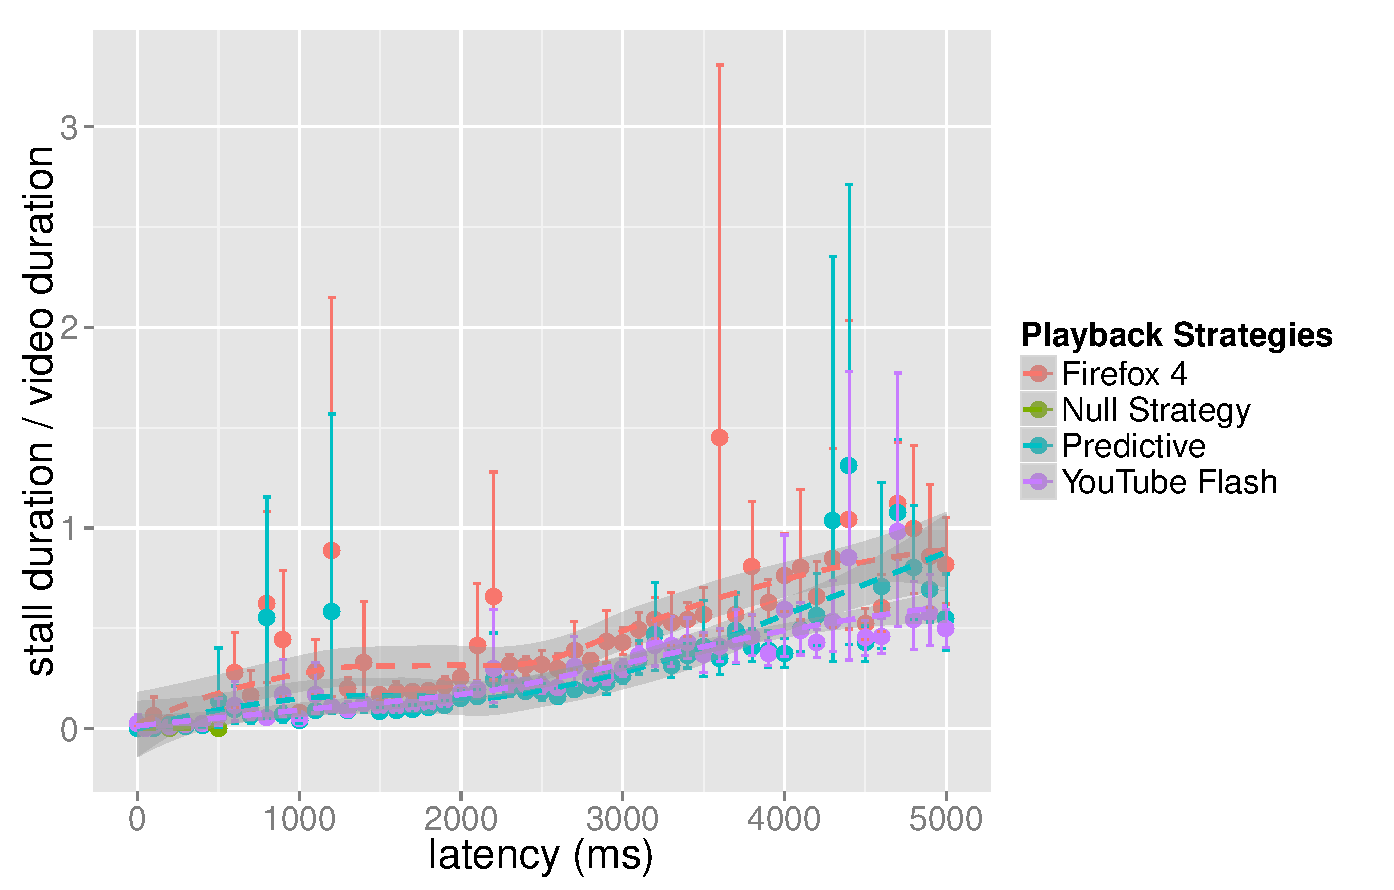
\includegraphics[width=0.9\textwidth]{images/R-playbackemulation-stallduration-latency.pdf}
	\caption{Stalling duration in relation to transmission latency with a local polynomial least-squares fit.}
\label{c3:fig:eval-latency-stallingtime}
\end{figure}

Figure~\ref{c3:fig:eval-latency-stallingtime} depicts the relation between the added latency and the stalling duration of the playback strategies. The stalling time increases as expected with the additional latency, but Firefox's strategy seems to have a slight edge during high latency. Overall, the stalling duration quickly reaches a length comparable to the actual video duration and even surpassing that. Someone watching a stream under this condition might find this not acceptable any longer.

\begin{figure}[htbp]
	\centering
	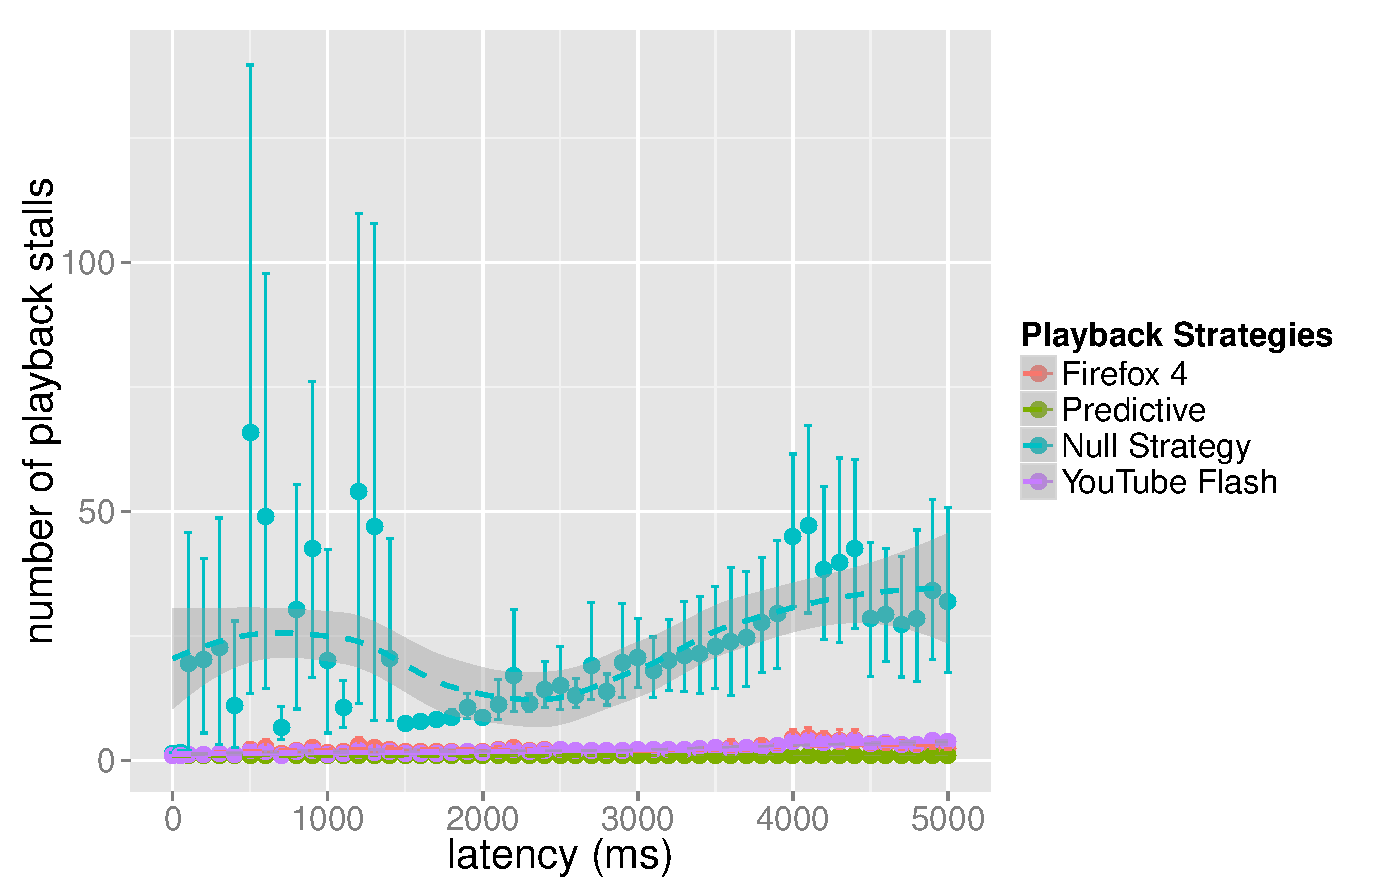
\includegraphics[width=0.9\textwidth]{images/R-playbackemulation-stallnumber-latency.pdf}
	\caption{Number of stalls in relation to transmission latency with a local polynomial least-squares fit.}
\label{c3:fig:eval-latency-numstalls}
\end{figure}

Figure~\ref{c3:fig:eval-latency-numstalls} additionally shows number of stalling events occurring during the playback with the null strategy at the high end and the predictive strategy just showing the expected single stall before playback start.

\begin{figure}[htb]
	\centering
	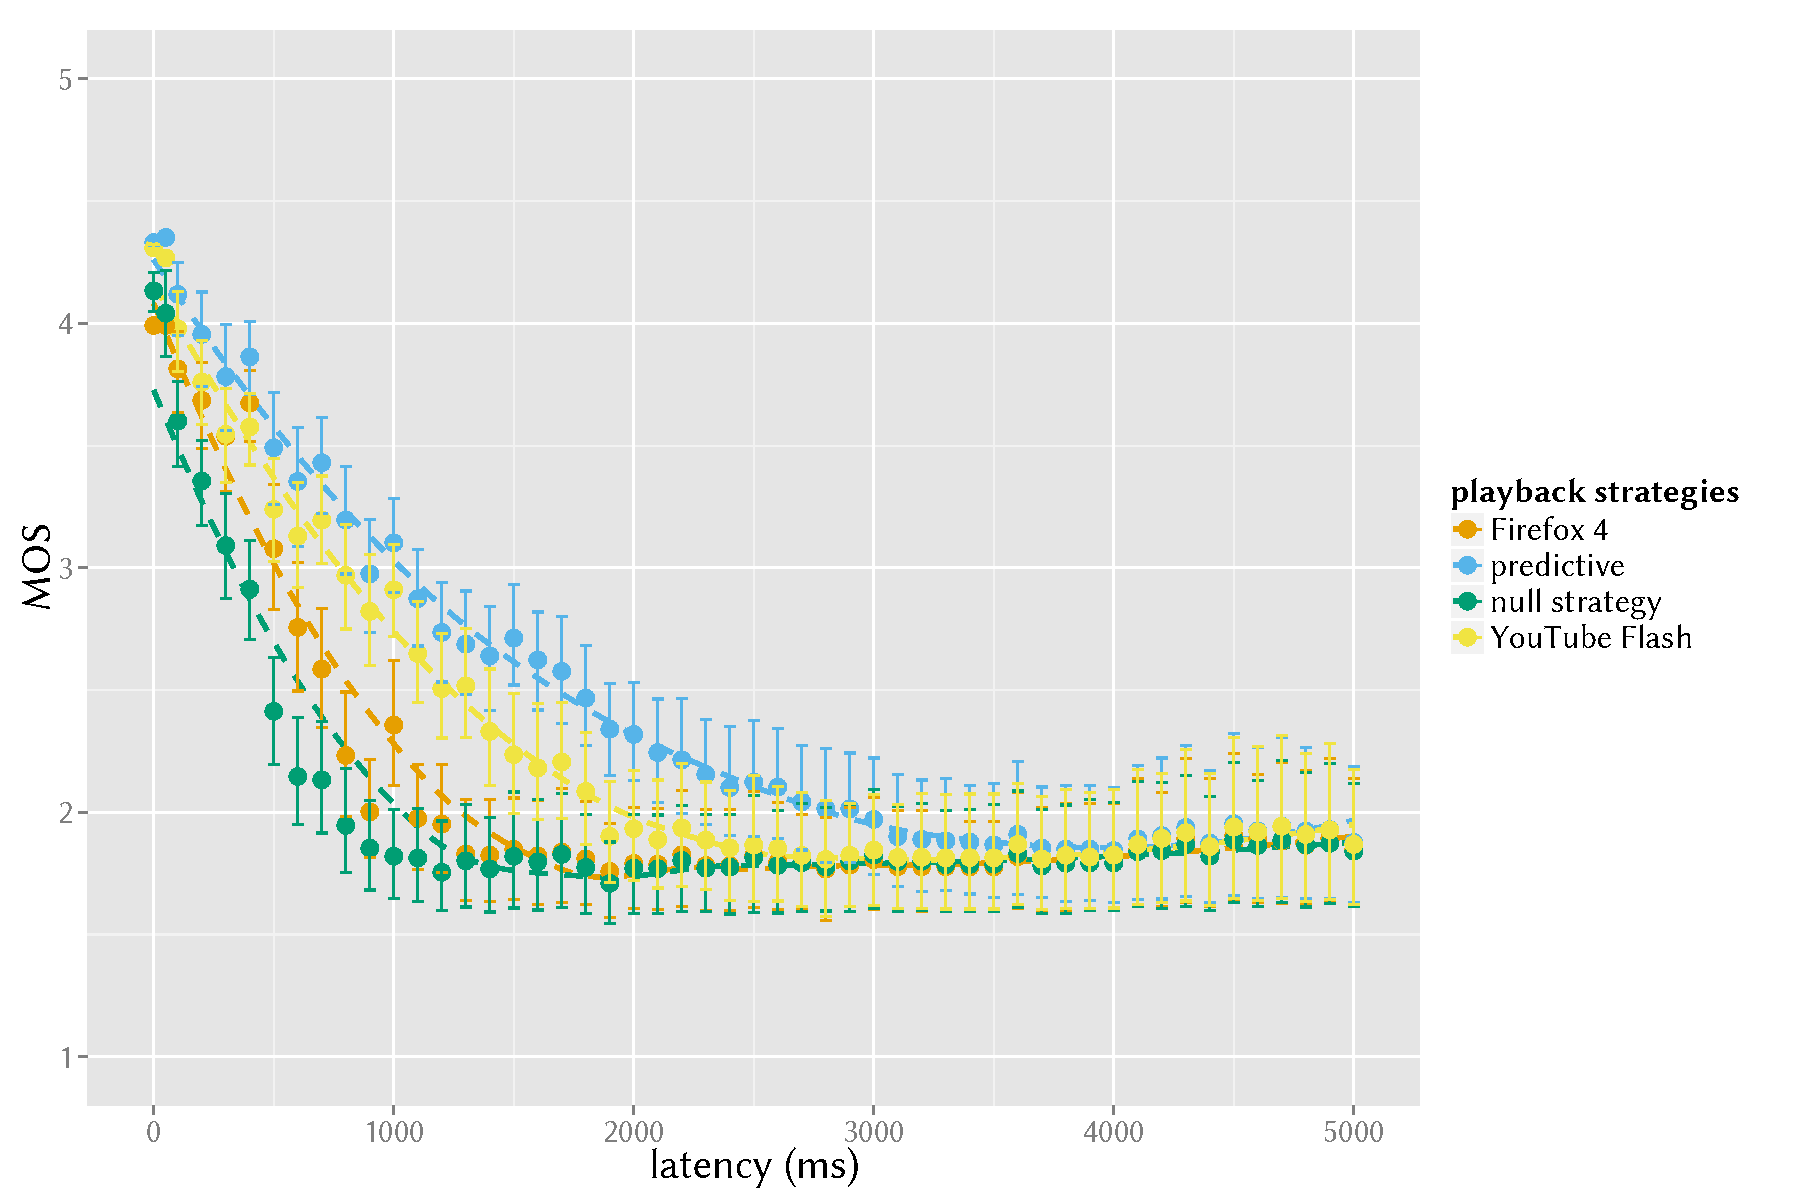
\includegraphics[width=0.9\textwidth]{images/R-playbackemulation-qoe-latency.pdf}
	\caption{Calculated \acrshort{MOS} for the latency measurement series.}
\label{c3:fig:eval-latency-qoe}
\end{figure}

Using the model from Equation~\ref{c3:eqn:hossfeld-stalling-model} the \gls{QoE} is calculated for this series and depicted in Figure~\ref{c3:fig:eval-latency-qoe}. The \gls{MOS} quickly drops below a value of $3$, which is generally accepted as still being of fair quality, and stays around $2$ for the most portion of the latency series. Starting at around \SI{3000}{\milli\second} of latency all four strategies achieve virtually the same poor quality, according to this model. But, especially between \SI{1000}{\milli\second} and \SI{2000}{\milli\second} the difference in quality of these strategies is visible, with both the theoretical predictive and the YouTube strategy reaching a much higher \gls{MOS} than the other two.

Overall, it can be said that in this specific latency scenario the real world playback strategies seem to honor the fact that more video interruptions lead to a worse experience than fewer but longer stalling events. Through mobility and handovers mobile devices fairly commonly experience short bursts of latency of several seconds. According to the measurement series, the resulting stalling behavior could still very well be bearable for streaming users if the latency does not reach too high values on average. For example, at \SI{1000}{\milli\second} latency a \gls{MOS} of $3$ could still be easily achievable.


%%
\subsubsection{Loss Measurement Series}

In the loss measurement series, uncorrelated and uniformly distributed loss was added in both the uplink and the downlink direction. The loss was incrementally increased in \SI{0.5}{\percent} steps up to a total additional loss of \SI{12.5}{\percent}. About \SI{4}{\percent} of the individual experiments did not finish correctly, and the video was not completely transmitted. This was caused by the \gls{TCP} stack, which at some point terminated the connection after too many packets were lost back to back, and curl giving up after several retries. This unpredictability and failure rate also leads to the high variability seen in the results of the loss measurement series. Nonetheless, a certain trend can still be derived from the results. Again, five experiments for each entry with corresponding error bars are conducted.


\begin{figure}[htbp]
	\centering
	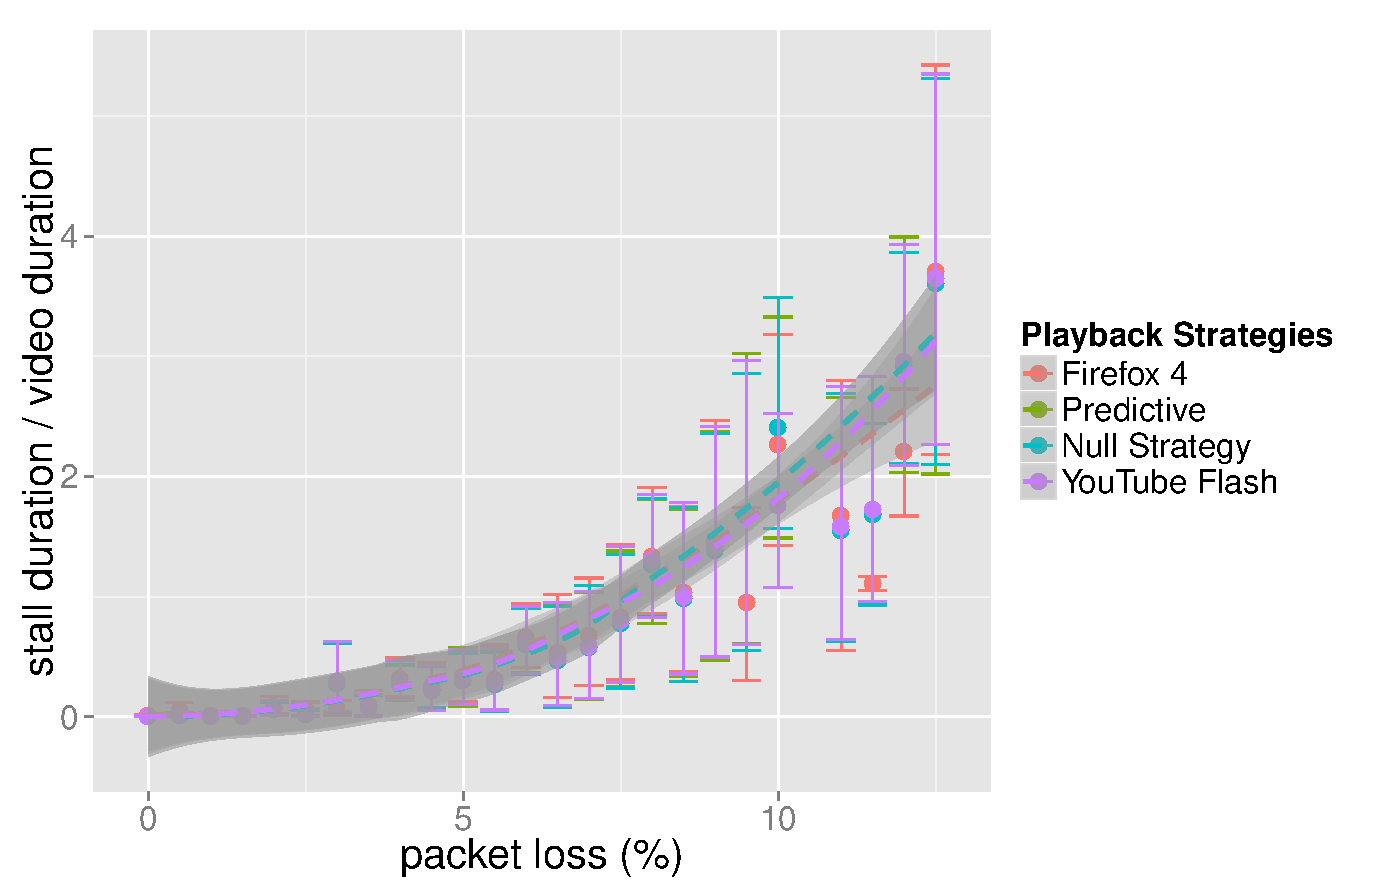
\includegraphics[width=0.9\textwidth]{images/R-playbackemulation-stallduration-loss.pdf}
	\caption{Stalling duration in relation to the packet loss with a local polynomial least-squares fit.}
\label{c3:fig:eval-loss-stallingtime}
\end{figure}

Figure~\ref{c3:fig:eval-loss-stallingtime} shows the resulting relative stalling duration in the packet loss measurement series. Loss of up to about \SI{2.5}{\percent} seems to have no discernible impact on the streaming process. Anything beyond this point sees a large increase in the stalling duration. With a relative stalling duration of almost four times the actual video length at \SI{12.5}{\percent} packet loss any streaming attempt is practically rendered unusable. Also, all four tested playback strategies handle high loss equally worse, with the exception of some Firefox results producing a lower stalling duration.

This general behavior could hint to the transport protocol's reliable transport feature, catching any occurring loss. However, the detection and retransmission of lost segments takes time and leads to a bursty increase in latency. It also represents a possible reason of the increased stalling time. 

At least it can be safely assumed that in actual production networks high values of packet loss are usually less likely to occur than high latency. The only major source of packet loss should be network congestion, which should only occur in moments of high network load. Therefore, it can be expected that playback strategies are better optimized for scenarios with high latency than loss.

\begin{figure}[htbp]
	\centering
	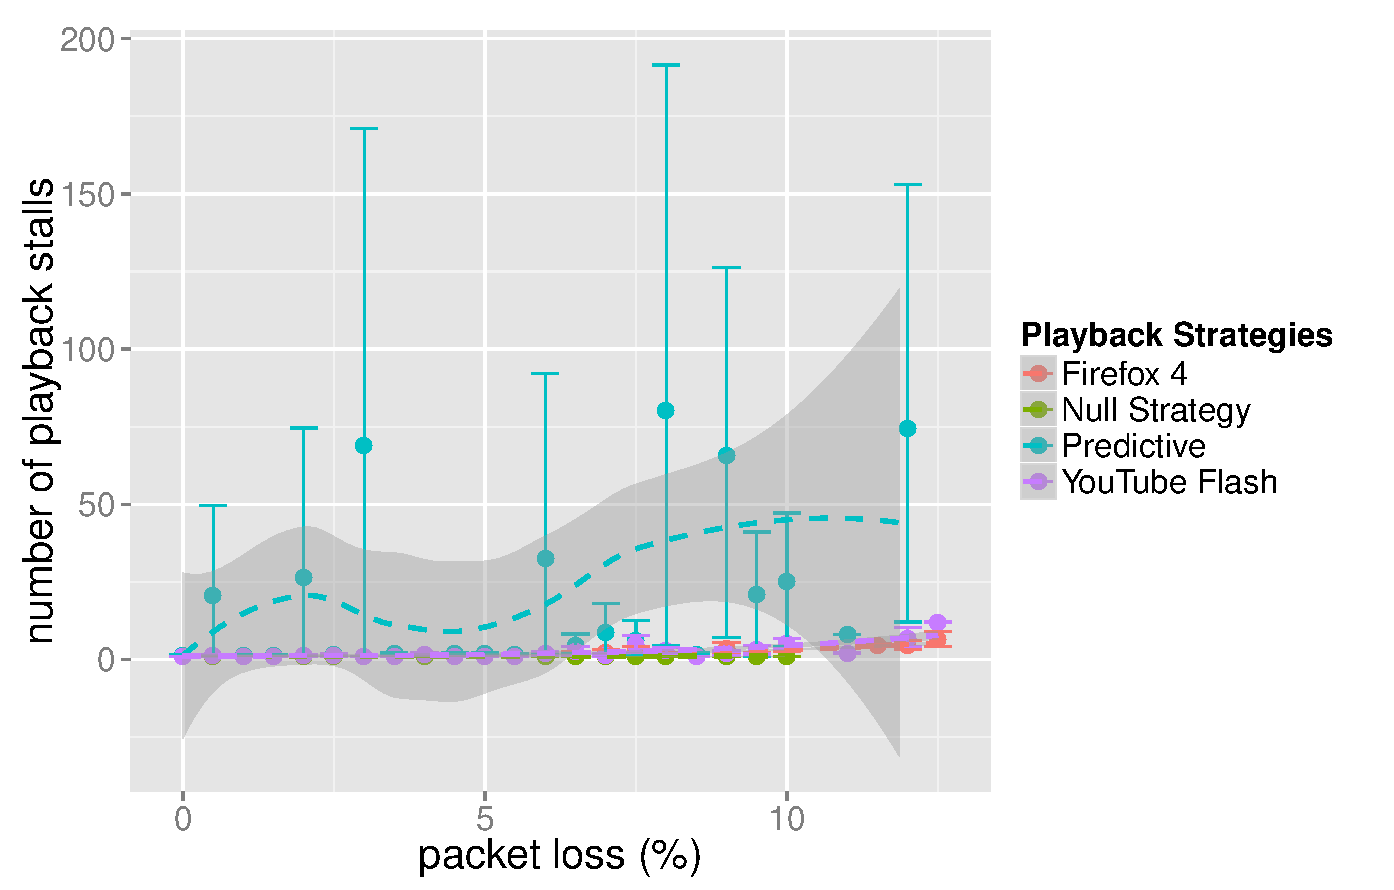
\includegraphics[width=0.9\textwidth]{images/R-playbackemulation-stallnumber-loss.pdf}
	\caption{Number of playback stalls in relation to packet loss with local polynomial least-squares fit.}
\label{c3:fig:eval-loss-numstalls}
\end{figure}

Figure~\ref{c3:fig:eval-loss-numstalls} clearly shows the extremity of the null strategy in terms of the number of experienced stalls compared to any other strategy. The same loss measurement series is used as basis here. The null strategy runs into two orders of magnitude more stalling phases than the three other strategies. The number of stalling events of the three other strategies remain relatively low. But the individual stalling events will therefore be rather lengthy ones when keeping the total stalling duration in mind. Therefore, in the packet loss scenario the factor that will degrade \gls{QoE} the most seems to be the duration of the stalling events but not their number, with the exception of the null strategy.

\begin{figure}[htb]
	\centering
	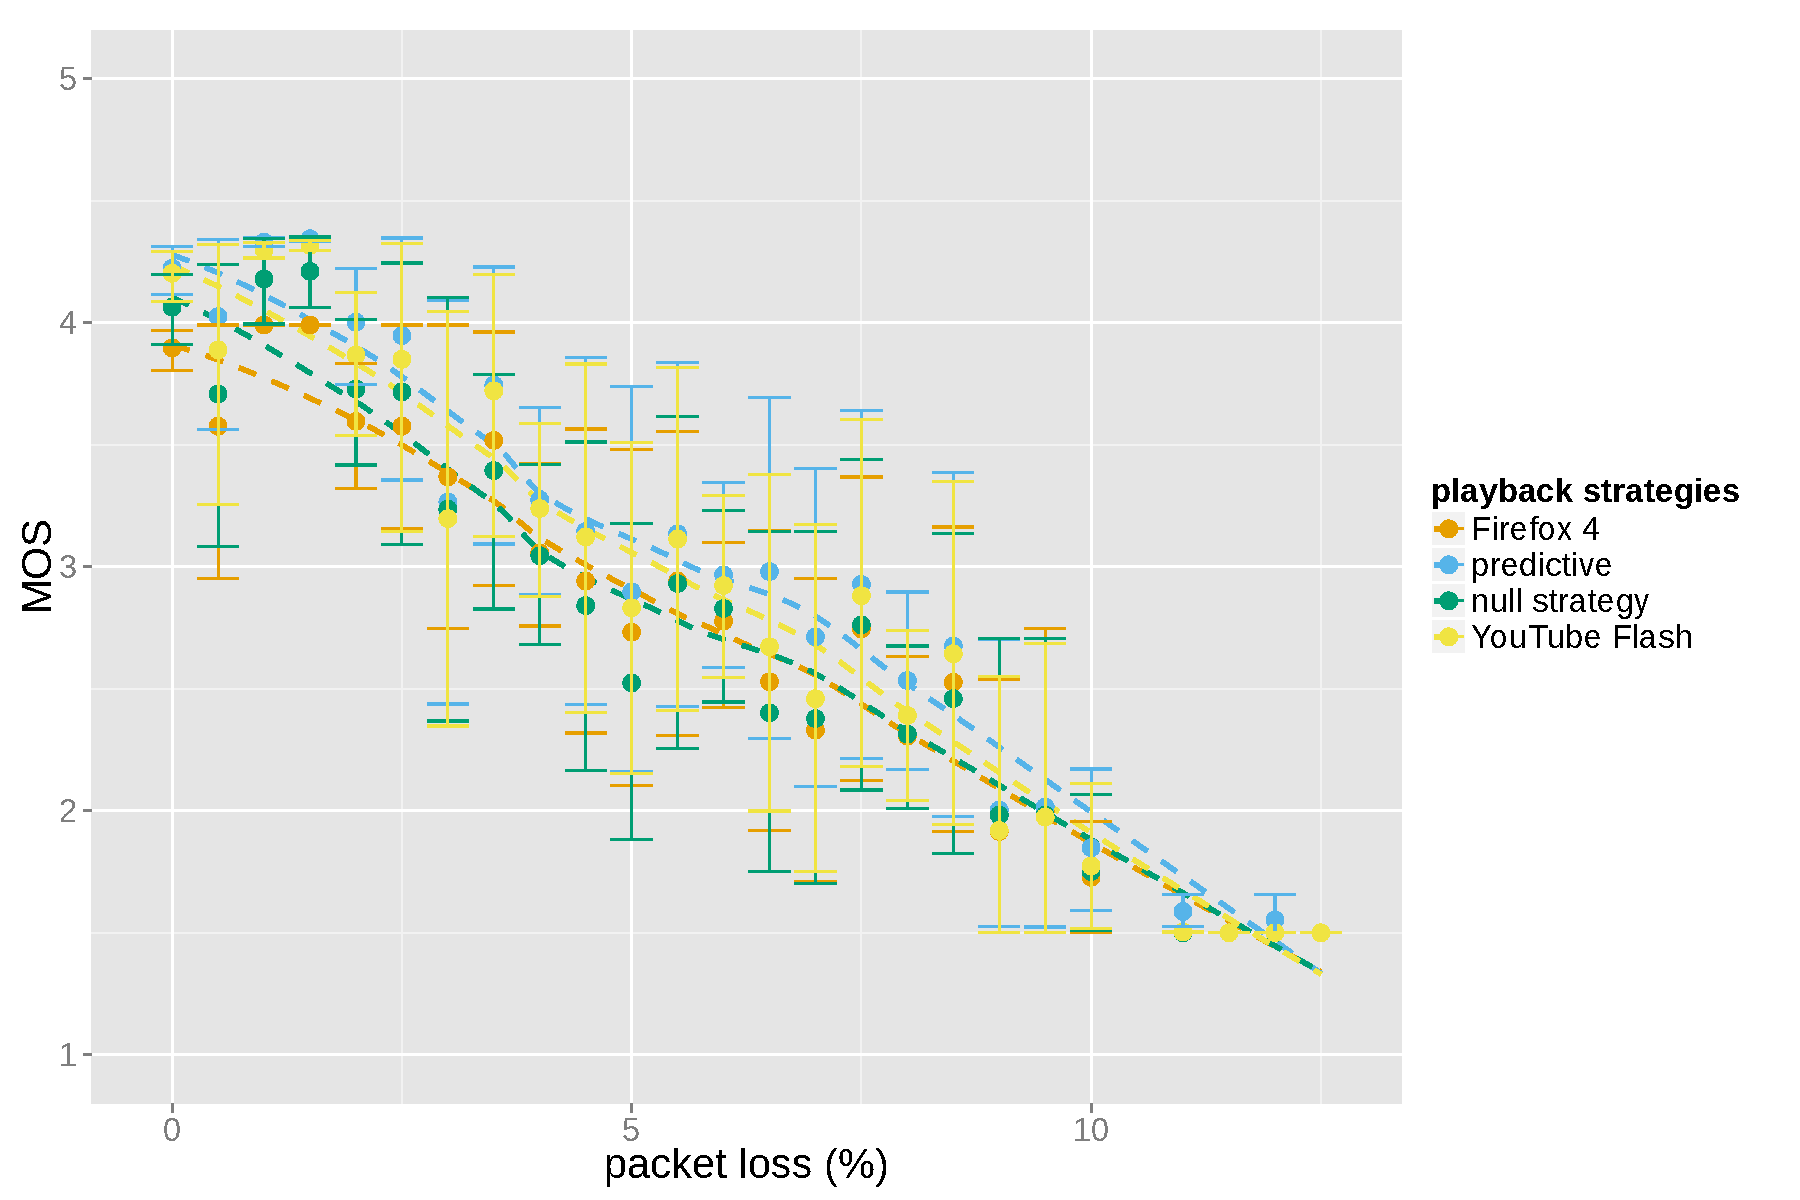
\includegraphics[width=0.9\textwidth]{images/R-playbackemulation-qoe-loss.pdf}
	\caption{Calculated \acrshort{MOS} for the loss measurement series.}
\label{c3:fig:eval-loss-qoe}
\end{figure}

Looking at the \gls{QoE} of the loss series, displayed in Figure~\ref{c3:fig:eval-loss-qoe}, the difference in \gls{MOS} between the playback strategies is much smaller than the one observed in the latency series. Additionally, the \gls{MOS} degradation happens much more slowly and evenly dispersed across the loss values. A \gls{MOS} of $3$ is only undercut at around \SI{5}{\percent} packet loss. But the fluctuations between the individual experiments is rather large in this series, often giving results $2$ \gls{MOS} apart for the same packet loss percentage, making loss a very unpredictable factor.

All in all, when planning a network for streaming applications, the maximum loss should be kept below the \SI{2.5}{\percent} mark to achieve reasonable streaming quality. All the existing strategies already seem to work rather well for typically experienced network \gls{QoS} scenarios. Only when extraordinary network conditions are present the strategies break down. But this is not different to many other network applications, which work best with pristine \gls{QoS}.





%% original python plots
% \begin{figure}[htb]
%     \centering
%     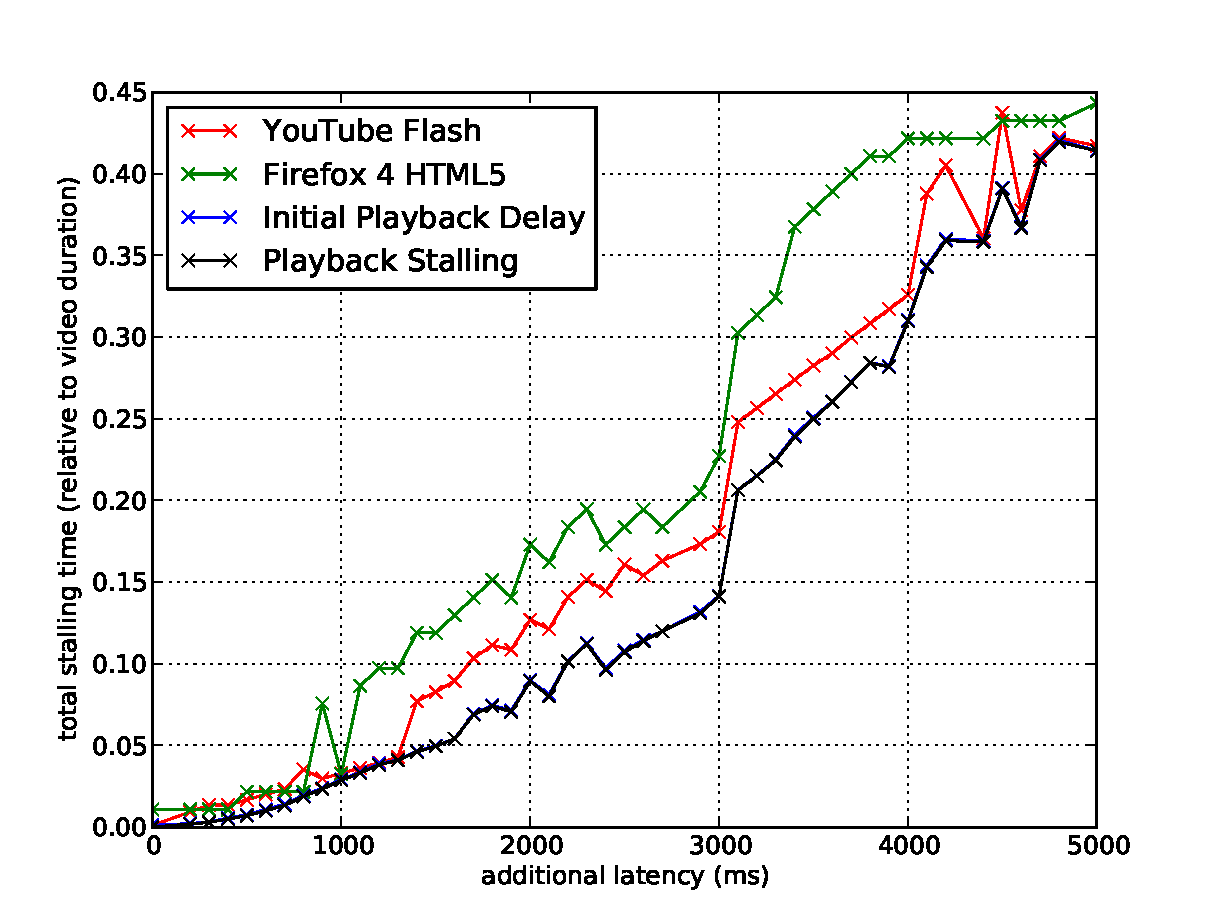
\includegraphics[width=\textwidth]{images/eval-latency-stallingtime.pdf}
%     \caption{Stalling duration in relation to transmission latency.}
%     \label{c3:fig:eval-latency-stallingtime}
% \end{figure}

% \begin{figure}[htb]
%     \centering
%     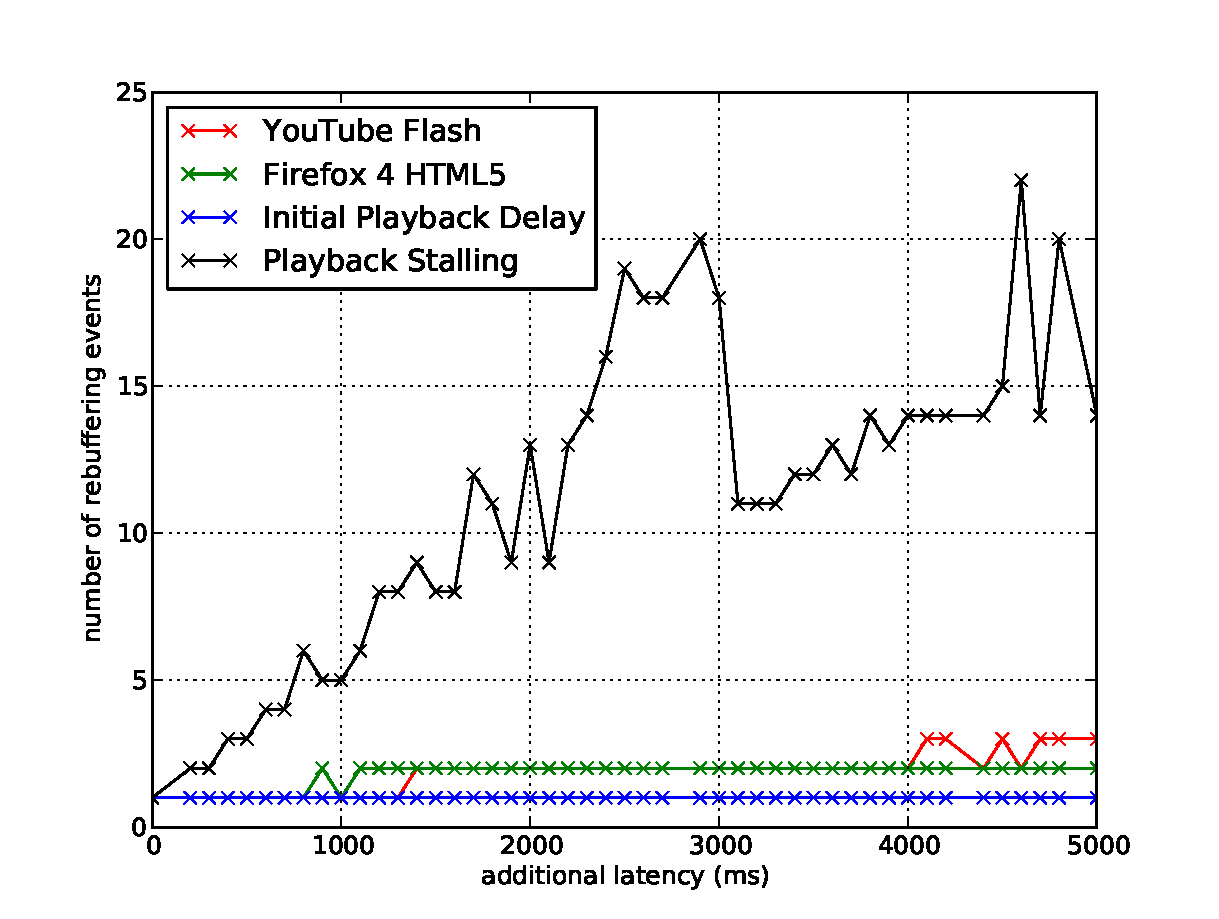
\includegraphics[width=\textwidth]{images/eval-latency-frequency.pdf}
%     \caption{Number of stalls in relation to transmission latency.}
%     \label{c3:fig:eval-latency-numstalls}
% \end{figure}

% \begin{figure}[htb]
%     \centering
%     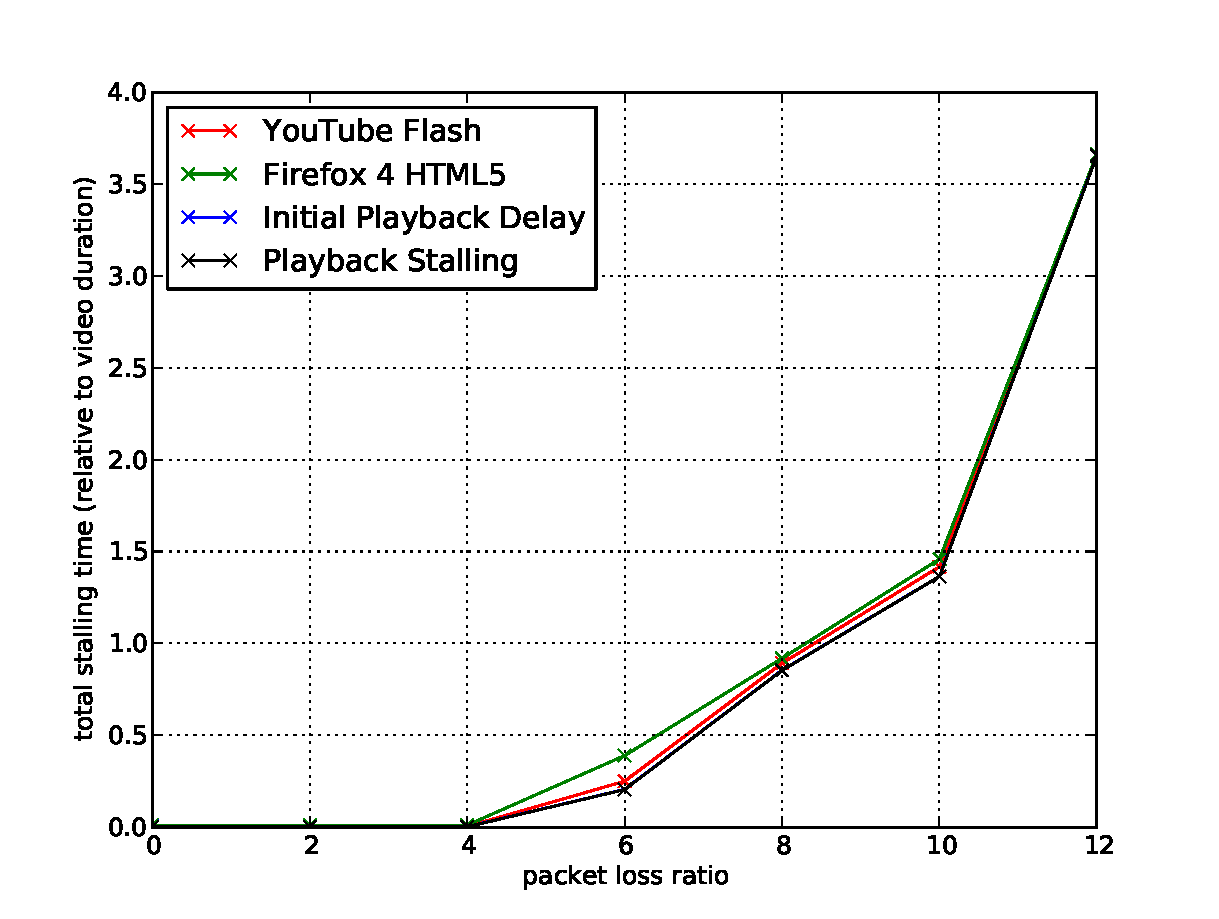
\includegraphics[width=\textwidth]{images/eval-loss4mb-stallingtime.pdf}
%     \caption{Stalling duration in relation to packet loss.}
%     \label{c3:fig:eval-loss-stallingtime}
% \end{figure}

% \begin{figure}[htb]
%     \centering
%     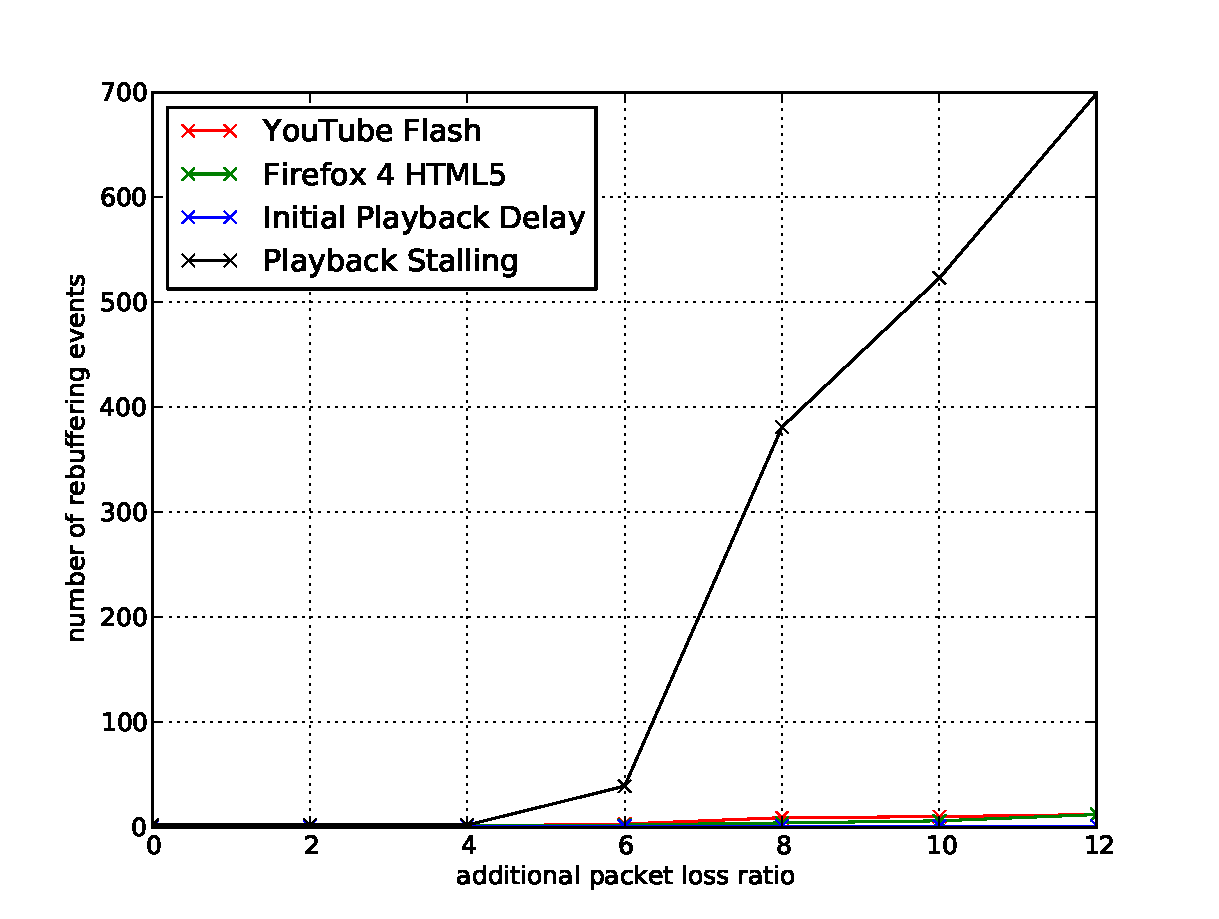
\includegraphics[width=\textwidth]{images/eval-loss4mb-frequency.pdf}
%     \caption{Number of playback stalls in relation to packet loss}
%     \label{c3:fig:eval-loss-numstalls}
% \end{figure}


% \begin{figure}[htbp]
%     \centering
%     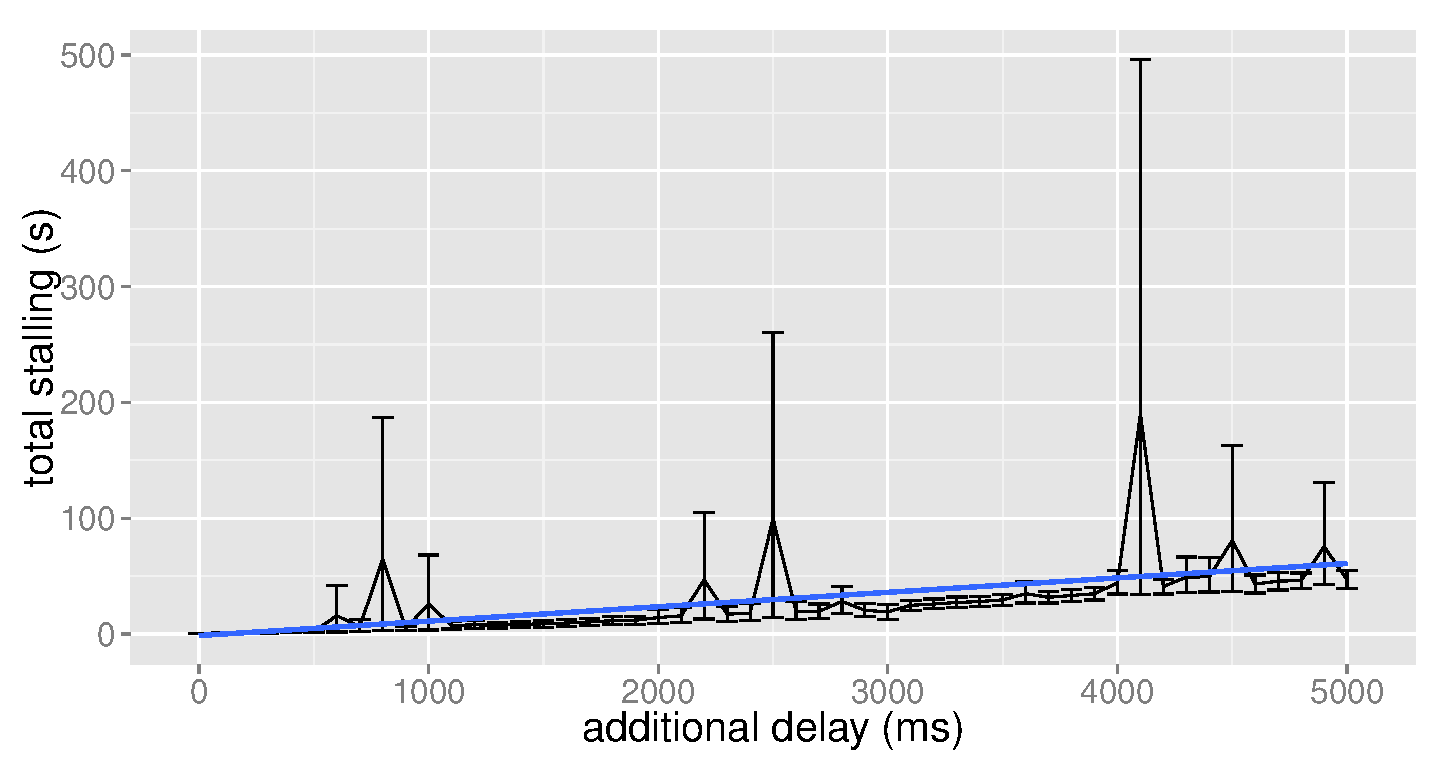
\includegraphics[width=\textwidth]{images/R-delayseries.pdf}
%     \caption{Total buffering time and linear smooth for degraded network parameter scenarios. Latency Graph.}
%     \label{c3:fig:delayseries}
% \end{figure}

% \begin{figure}[htbp]
%     \centering
%     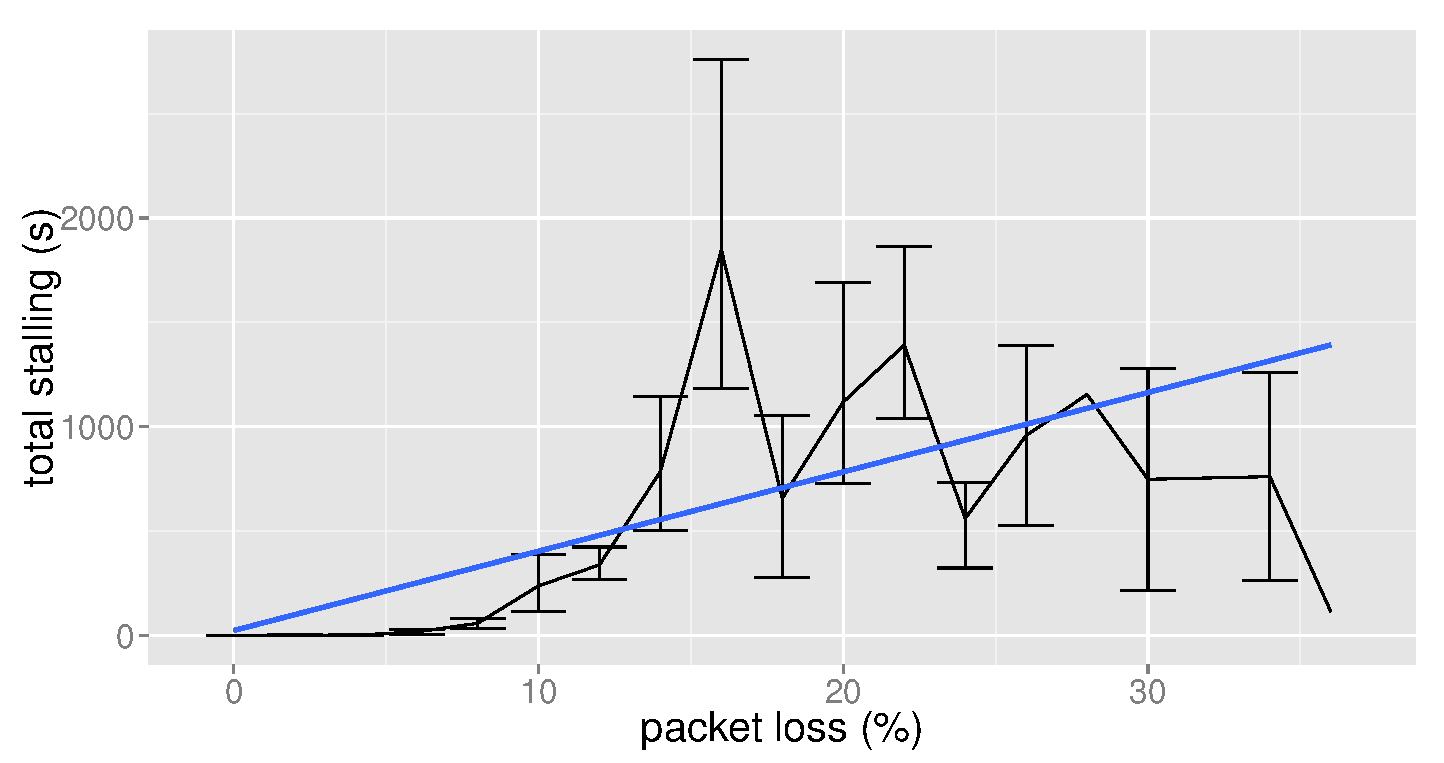
\includegraphics[width=\textwidth]{images/R-lossseries.pdf}
%     \caption{Total buffering time and linear model for degraded network parameter scenarios. Loss Graph.}
%     \label{c3:fig:lossseries}
% \end{figure}